%\documentclass[preprint,12pt]{elsarticle}
% uncomment for submission to NIM A
\documentclass[review,number,sort&compress]{elsarticle}
\usepackage{lineno}
\linenumbers


\usepackage{amssymb}
\usepackage{amsmath}
\usepackage{float}
\usepackage{listings}
\usepackage{amssymb}
\usepackage{tabularx}
\usepackage{tikz}
\usepackage{float}
\usepackage{mathtools}
%\usepackage{minted}
\usepackage[colorinlistoftodos]{todonotes}
\usepackage[ruled,vlined]{algorithm2e}
\usepackage{hyperref}
\usepackage{enumerate}
\usepackage[shortlabels]{enumitem}
\usepackage{amssymb}
\usepackage{subfig}
\usepackage{makecell}
\usepackage{array}
\usepackage{multirow}
\usepackage{mathpazo}
%\usepackage{multicol}
%\usepackage{siunits}
\usepackage{siunitx}
\usepackage{graphicx}
\usepackage{longtable}
\usepackage[toc,page]{appendix}
\usepackage{booktabs}
\usepackage{tabularx}
\usepackage{adjustbox}
\usepackage[section]{placeins}
\usepackage{pdflscape}
\usepackage[utf8]{inputenc}
\usepackage[T1]{fontenc}

\usepackage{natbib}
\bibliographystyle{unsrtnat}


\setlength{\marginparwidth}{4cm}
\usepackage{todonotes}
\newcommand{\inner}[2]{\langle #1 | #2 \rangle}
\newcommand{\R}{\mathbb{R}}
\newcommand{\wij}{W_{ij}}
\newcommand{\loss}{\mathcal{L}}

\journal{Nuclear Instruments and Methods
in Physics Research Section A: Accelerators, Spectrometers,
Detectors and Associated Equipment}

\begin{document}

\begin{frontmatter}

%% \title{Title\tnoteref{label1}}
%% \tnotetext[label1]{}
%% \author{Name\corref{cor1}\fnref{label2}}
%% \ead{email address}
%% \ead[url]{home page}
%% \fntext[label2]{}
%% \cortext[cor1]{}
%% \address{Address\fnref{label3}}
%% \fntext[label3]{}

\title{Unsupervised Learning  for Identifying  Events in Active Target  Experiments}

%% use optional labels to link authors explicitly to addresses:
%% \author[label1,label2]{}https://www.overleaf.com/project/5e73f990fcbd310001959b01
%% \address[label1]{}
%% \address[label2]{}

\author{R.~Solli}
\address{Expert Analytics AS, Tordenskiolds gate 6, 0160, Oslo, Norway}
\address{Department of Physics, University of Oslo, POB 1048 Oslo, N-0316 Oslo, Norway}

\author{D.~Bazin}
\address{Department of Physics and Astronomy and Facility for Rare Ion Beams and National Superconducting Cyclotron Facility, Michigan State University, East Lansing, MI 48824, USA}
\author{M.P.~Kuchera}
\address{Department of Physics, Davidson College, Davidson, North Carolina, USA}
\author{R.R.~Strauss}
\address{Department of Mathematics and Computer Science, Davidson College, Davidson, North Carolina, USA}

\author{M.~Hjorth-Jensen}
\address{Department of Physics and Astronomy and Facility for Rare Ion Beams and National Superconducting Cyclotron Facility, Michigan State University, East Lansing, MI 48824, USA}
\address{Department of Physics and Center for Computing in Science Education, University of Oslo, POB 1048 Oslo, N-0316 Oslo, Norway}
\ead{hjensen@frib.msu.edu}
\ead[url]{http://mhjgit.github.io/info/doc/web/}


\begin{abstract}
% Modified by DB (6/8/2020)
This article presents novel applications of machine learning methods to the problem of event separation in an active target detector, the Active-Target Time Projection Chamber (AT-TPC) \cite{Bradt2017}. 
The overarching goal is to identify classes of events in the early stages of the data analysis, thereby improving its efficiency by limiting the computationally expensive processing to events of interest only, which are often not the most abundant.
%Machine learning presents an interesting avenue for researchers operating the AT-TPC, as traditional analysis methods of AT-TPC data are computationally expensive and have to fit all tracks against the event type of interest. The latter presents a considerable challenge when either the space of reactions is not known prior to the analysis, or the event type of interest is not the most abundant. 
The application of unsupervised clustering  algorithms to the analysis of two-dimensional projections of particle tracks from a resonant proton scattering experiment on $^{46}$Ar is introduced. We explore the performance of autoencoder neural networks and a pre-trained VGG16 \cite{Simonyan2014} convolutional neural network.
%on two tasks: a semi-supervised classification task and the unsupervised clustering of particle tracks. 
%On the semi-supervised task, we find that a logistic regression classifier trained on small labelled subsets of the latent space of these models perform very well, both on simulated and real data. On the clustering task, 
We find that a $K$-means algorithm applied to the simulated data in the VGG16 latent space forms almost perfect clusters. Additionally, the VGG16+K-means approach finds high purity clusters of proton events for real experimental data. We also explore the application of neural networks to clustering by implementing a mixture of autoencoders algorithm, with improved results on real data. 




\end{abstract}

%%Graphical abstract
\begin{graphicalabstract}
%\includegraphics{grabs}
\end{graphicalabstract}

%%Research highlights
\begin{highlights}
\item Research highlight 1
\item Research highlight 2
\end{highlights}

\begin{keyword}
%% keywords here, in the form: keyword \sep keyword

%% PACS codes here, in the form: \PACS code \sep code

%% MSC codes here, in the form: \MSC code \sep code
%% or \MSC[2008] code \sep code (2000 is the default)

\end{keyword}

\end{frontmatter}

\section{Introduction}\label{sec:intro}



The AT-TPC \cite{Bradt2017} is a novel type of detector designed specifically for nuclear physics experiments where the energies of the recoiling particles are very low compared to the energy required to escape target material. The luminosity of nuclear physics experiments performed with fixed targets is directly proportional to the amount of material encountered by the beam. On the other hand, for several classes of experiments the detection of recoil particles is paramount, therefore limiting the target thickness. In addition, the properties of the recoil particles are modified while traversing the target material, affecting the resolutions that can be achieved. This necessary balance between luminosity and resolution is particularly difficult when performing experiments with rare isotope beams, because of the low intensities available. 

The concept of active targets aim at mitigating this compromise, by turning the target itself into a detector \cite{BECEIRONOVO2015}. Most active target detectors such as the AT-TPC are composed of a time projection chamber (TPC) where the detector gas is at the same time the target material. Recoil particles that originate from a nuclear reaction between a beam nucleus and a gas nucleus can be tracked from the vertex of the reaction to their final position inside the active volume of the target. Their properties can therefore be measured without any loss of resolution regardless of the amount of material traversed by the beam. At the same time, the detection efficiency is dramatically increased by the very large solid angle covered in this geometry. A direct consequence of this concept is the inclusiveness of the experimental data recorded by this type of detector: any nuclear reaction happening within the target is recorded. Although this sounds like an advantage from the scientific point of view, it poses great challenges during the analysis phase, that are reminiscent of bubble chamber times and on par with event classification challenges in particle physics today, see for example the recent review of Mehta {\em et al.} \cite{mehta2019}. More often than not, the reaction channel of interest has one of the lowest cross sections, therefore the physicist is faced with the task of sorting out the corresponding events from the ``background" of other reaction channels. 

% motivating ML work:
Because TPCs produce 3-dimensional images of charged particle tracks, the event identification task is often akin to a visual inspection (akin to analysis in the bubble chamber era), which is not practical nowadays because of the large quantities of data. Machine learning techniques then appear as a promising prospect, in particular in the image recognition domain where much progress has been made recently \cite{mehta2019}. In addition, some ML algorithms offer new possibilities such as the potential discovery of unforeseen phenomena that would have been missed by more traditional analysis methods. Prior work has demonstrated the ability to apply supervised classification machine learning methods to AT-TPC data when a labeled training set is available, whether through hand-labeled data or labeled simulated data (a {\em transfer learning} application) \cite{Kuchera2019}. In some experiments, a labeled dataset is unavailable. This could be  due to the inability to hand-label events, or the case where one does not know a priori the types and behaviors of the reactions present in the detector in order to generate a labeled, simulated dataset. In the latter case, there must also exist a validation dataset of real data, still requiring the ability to label a subset of the real data. The unsupervised separation of event types, or {\em clustering}, based on a set of ML algorithms is hereby examined, using experimental data recorded by the AT-TPC during its commissioning experiment from a radioactive $^{46}$Ar beam reacting on an isobutane target composed of proton and carbon nuclei. 

\section{Experimental Details} 
\label{Sec:Exp}
The goal of the experiment was to measure the evolution of the elastic and inelastic cross sections between $^{46}$Ar and protons as a function of energy (the {\em excitation function}), and observe resonances in the composite system $^{47}$K that correspond to analog states in the nucleus $^{47}$Ar. Spectroscopic information can then be obtained from the shape and amplitude of the observed resonances \cite{Bradt2018}. 
The experiment was performed at the National Superconducting Cyclotron Facility (NSCL) where a $^{46}$Ar beam was produced via fragmentation of a $^{48}$Ca beam on a $^9$Be target at about 140 MeV/u. The $^{46}$Ar isotopes were then filtered, thermalized, and finally re-accelerated to 4.6 MeV/u by a linear accelerator. This scheme was used to produce a low-emittance beam, which is necessary to guarantee a good energy resolution in the excitation function. Because the  $^{46}$Ar beam particles lose energy as they traverse the target gas volume, the position of the reaction vertex along the beam axis is directly related to the energy at which the reaction occurs. This allows the AT-TPC to measure the excitation function over a wide range of energies from a single beam energy.

The detector was placed inside the bore of a MRI solenoid energized to $\sim 2$ Tesla. This axial magnetic field served the purpose of bending the trajectories of the recoil particles in order to i) increase their length and ii) provide a measurement of their bending radius, directly related to their magnetic rigidity. Because the recoil particles travel in gas, they slow down and eventually stop, therefore their trajectories are described by 3-dimensional spirals (see \cite{Bradt2017}). One of the difficulties encountered in the analysis is that the shape of these spirals does not have an analytical form because it follows the energy-loss profile of the particles. It therefore needs to be simulated via an integration, which is numerically costly. Other difficulties are related to several experimental effects that deteriorate the quality of the data, namely saturation and cross-talk effects, as well as random noise. 

The method used in \cite{Bradt2018} to analyze the data followed a 3-phase sequence: cleaning, filtering and fitting. Traditional methods were used to perform each of these tasks, and ultimately extract the scientific information, but there were severe limitations and high computational costs that become prohibitive in data sets larger by an order of magnitude. 
% Begin added by DB (06/10/2020)
The cleaning was performed using a combination of linear and circular Hough transforms on a 2-dimensional projection of the tracks \cite{Bradt2017}. The following filtering and fitting phases were performed simultaneously, by defining the cost function to the fitting algorithm as a sum of 3 $\chi^2$ components based on i) the position of the track in space, ii) the energy deposited on each pixel of the sensor plane, and iii) the location of the vertex of the reaction. While various fitting algorithms were tested, the most accurate was a Monte-Carlo algorithm that explored the 6-dimensional phase space of the particle's kinematics parameters, reducing it progressively at each iteration step until the desired accuracy was reached \cite{Bradt2017}. Although this algorithm ended up being the most accurate, it is extremely costly computationally because of the very large number of simulated tracks needed for each event. The filtering was performed by setting limits to the $\chi^2$ distributions, below which the events were assigned as proton scattering. This is a very inefficient method because it requires performing the fitting for all events, including those that are not of interest. Pioneering work on event identification using ML methods, namely the use of a pre-trained CNN, later showed that the filtering phase would better be performed using this type of technique \cite{Kuchera2019}. 
% End added by DB (06/10/2020)
In addition, \cite{Kuchera2019} demonstrated that the purity and statistics of the data are improved with the use of ML.

% From DB (06/19/2020)
From the experimenter's point of view, it is clear that the method used in \cite{Bradt2018} to identify and filter events is not the most efficient computationally. The ML methods explored in \cite{Kuchera2019} are a step forward, but they still rely on supervised learning methods that require data labeling, a time-consuming and error-prone process. The aim of the present study is to investigate unsupervised learning methods that bypass the labeling step, and form classes of events independently from the experimenter's input. The task of labeling the different classes is then much less time-consuming and can potentially lead to the discovery of unforeseen types of events.

\section{Data Preparation}

In this section we give a brief overview of the data, for a more in-depth consideration we refer the reader to \cite{Mittig2015}, \cite{Suzuki2012} and  \cite{Bradt2017a}. 

The AT-TPC data we studied for this work was recorded as charge time-series for each of the  the $\sim10^4$ detector pads.
In this representation, an event is a record of $512$ time-buckets for each of the $10^4$ detector pads. In our analysis, we represent each event as a downsampled 2D projection.
We chose to represent the data in 2D to facilitate the use of sophisticated image-recognition machine learning models, and this data representation was shown to successfully classify the events of this experiment in a supervised setting \cite{Kuchera2019}.
First, the time-series data was represented as a 3D point cloud, where each point contains the maximum charge in the time-series trace. We log-transform then min-max scale the charge, mapping the charge to the interval $[0, 1]$. The data is projected into 2D space by summing over the time-axis, then downsampled into an $128\times128$ pixel image.
%Additionally, we log-transform and normalize the data to the interval $[0, 1]$ for each point. The final representation for each event is a $128 \times 128$ matrix with each element ranging from $0$ to $1$.

One of the significant considerations for the analysis of AT-TPC data is to inject machine learning methods for track identification at the best point in the analysis pipeline.
Using raw data is advantageous as it provides an unbiased view of the event, but the data volume and noise levels might be prohibitive for analysis.
%On the opposite end of the pipeline, 
Therefore, incrementally add bias to the analysis by applying the algorithm further down the analysis pipeline.. With the benefit being that more pre-processing improves the signal-to-noise ratio, possibly improving model performance.
To explore this trade-off between model performance and pre-processing bias, we performed analysis on simulated, cleaned and raw events.

\begin{table}
\centering
\caption{Event class percentages for each of the datasets used in this analysis. The decrease in the "other" class of events from full to filtered data owes to the thresholding of events. If an event contains fewer than $20$ data-points it is discarded }\label{tab:class_distr}
\begin{tabular}{lccc}
\toprule
{} & Simulated & Full & Filtered \\
\midrule
$\%$ Proton & $50$ & $25.3$ & $27.6$ \\ 
$\%$ Carbon & $50$ & $12.0$ & $11.9$ \\
$\%$ Other & $0$ & $62.8$ & $60.1$ \\
\end{tabular}
\end{table}

\subsection{Simulated \texorpdfstring{${}^{46}$Ar}{46Ar}  events}\label{sec:data_sim}

A set of $N=40000$ simulated AT-TPC events per class were simulated from a ${}^{46}$Ar$(p, p)$ experiment with the \lstinline{pytpc} package developed by \citet{Bradt2017a}. %Using the same parameters {\color{blue} what parameters are you referring to? -MPK} as for the 
%Two simulated ${}^{46}$Ar$(p, p)$ experiment, a small set of $N=4000$ events per class was generated, as well as a larger set of $N=40000$ events per class. 

For validation, we set a subset of the simulated data to be labelled and treat the rest as unlabelled data. We choose this partition to be $15\%$ of each class. We denote this subset and its associated labels as $\gamma_L=(\boldsymbol{X}_L, \boldsymbol{y}_L)$, while the entire dataset which is identified as $\boldsymbol{X}_F$. Note that $\boldsymbol{X}_L \subset \boldsymbol{X}_F$.



\subsection{Raw \texorpdfstring{${}^{46}$Ar}{46Ar}  events}\label{sec:data_real}

The events analyzed in this section were retrieved from the ${}^{46}$Ar resonant proton scattering experiment recorded with the AT-TPC. 
While we denote these events as raw, it is important to note that what we mean is a raw 2D representation of peak-only events.

%The sensor plane in the AT-TPC is very sensitive, as such there is substantial noise in the ${}^{46}$Ar data. The noise can be attributed to structural noise from electronics cross-talk, and possible interactions with cosmic background radiation, as well as other sources of charged particles. Part of the challenge for this data then comes from understanding of the physics of the major contributing factors to this noise. \todo{I guess this paragraph can go. It reads very thesis-y, but I'm not sure what to do here to sensibly frame the raw data}

We display two different events from the ${}^{46}$Ar experiment in figure \ref{fig:samples}. The top row illustrates a carbon event with a large fraction of noise, while the bottom row shows a proton event nearly devoid of noise.

\begin{figure}[ht]
\centering
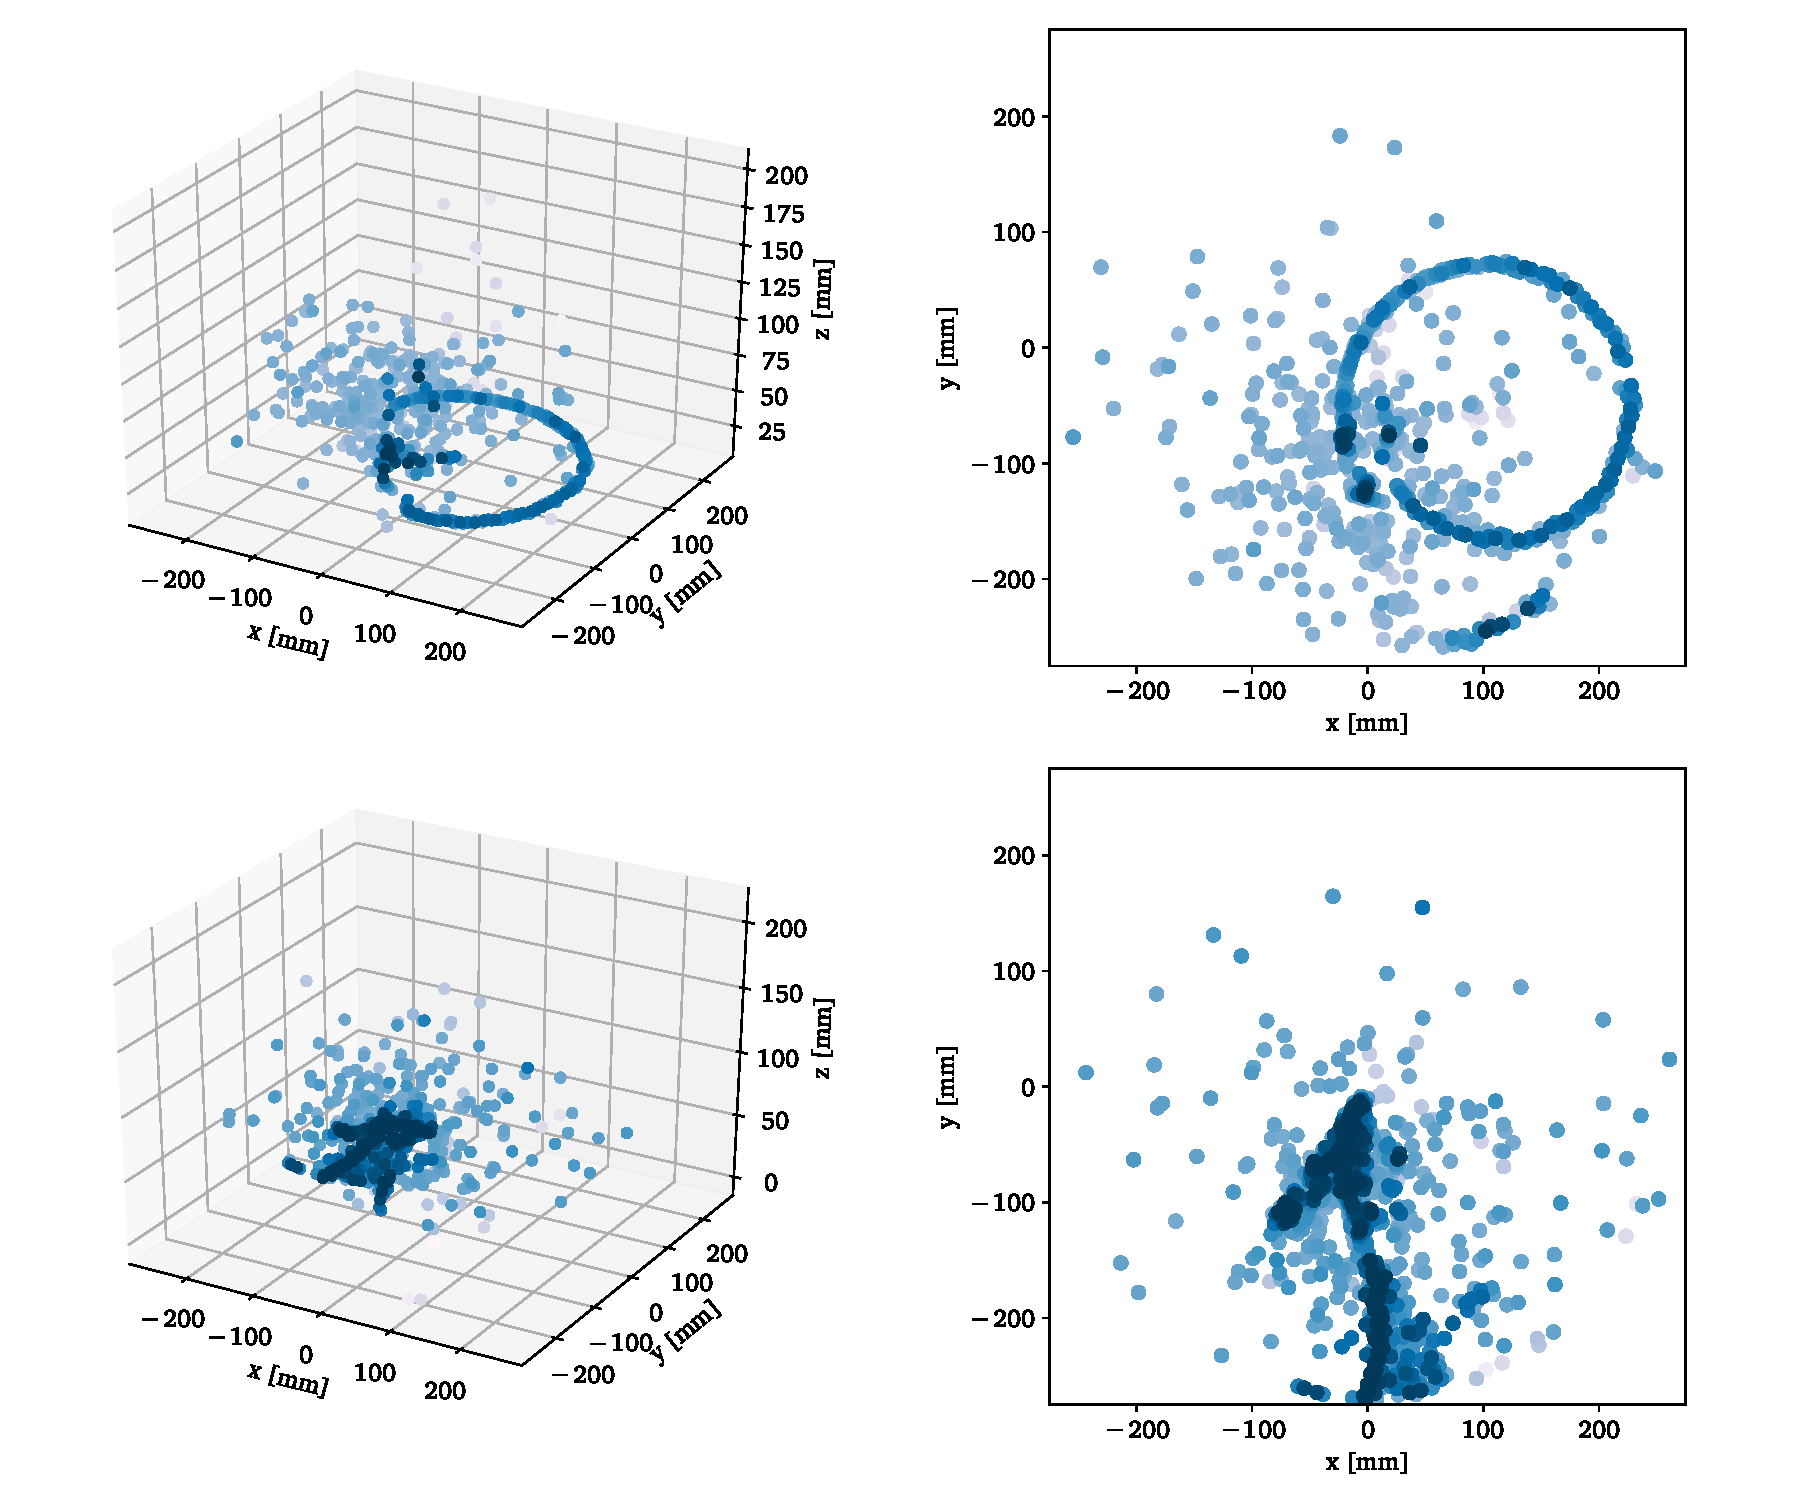
\includegraphics[width=\textwidth]{custom_work/examples_raw.pdf}
\caption[Displaying unfiltered events in 2D and 3D]{Two- and three-dimensional representations of two events from the ${}^{46}$Ar experiment. Each row is one event in two projections, where the color intensity of each point indicates higher charge values recorded by the detector.}\label{fig:samples}
\end{figure}

\subsection{Filtered \texorpdfstring{${}^{46}$Ar}{46Ar} events}\label{sec:filtered}


As we saw in the previous section, the detector picks up a significant amount of noise. We split the noise broadly in two categories,  one being random-uncorrelated noise and the second is structured noise. The former can be quite trivially removed with a nearest-neighbour algorithm that checks if a point in the event is close to any other. To remove the correlated noise, researchers at the NSCL developed an algorithm based on the Hough transform \cite{Newman1972}. This transformation is a common technique in computer vision, used to identify common geometric shapes like lines and circles, and has been used extensively in high-energy particle physics since the bubble-chamber era \cite{Hough:1959}.  %Essentially, the algorithm draws many lines (of whatever desired geometry) through each data-point and checks whether these lines intersect with points in the dataset. Locations in parameter space that generate many intersections then become bright spots, allowing us to filter away points that are not close to these points. These algorithms remove a large amount of the unstructured noise and are computationally rather cheap. \todo{Also pretty thesis-y language. Do not like}

We illustrate two filtered events in figure \ref{fig:samples_filtered}. These are the same events as shown in figure \ref{fig:samples}, but with the Hough and nearest neighbours filtering applied. 

\begin{figure}[ht]
\centering
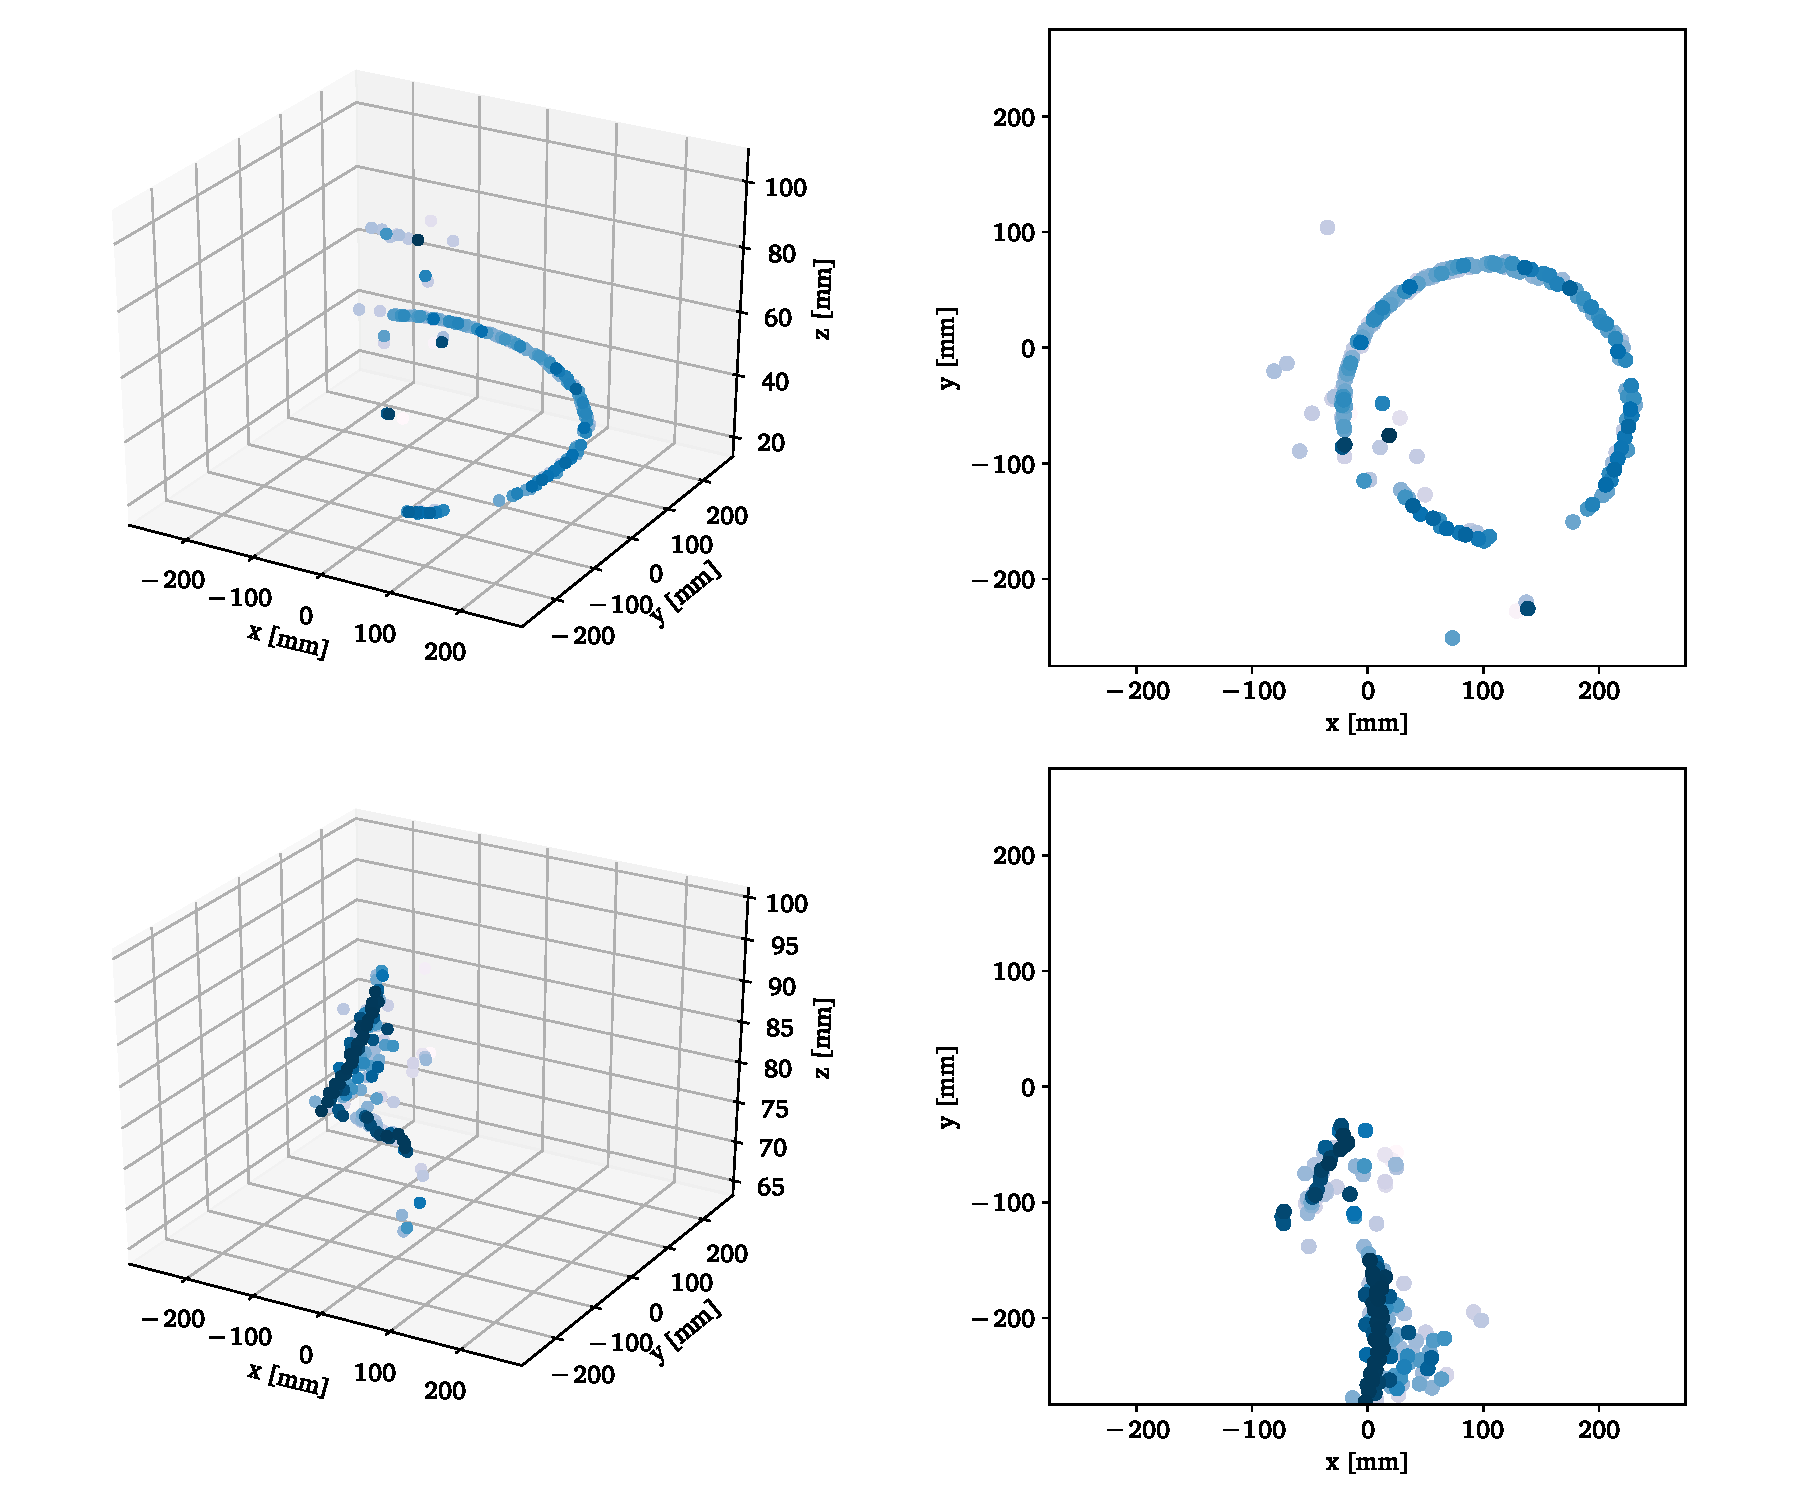
\includegraphics[width=0.9\textwidth, height=9cm]{custom_work/examples_filtered.pdf}
\caption[Displaying filtered events in 2D and 3D]{Two- and three-dimensional representations of two events from the ${}^{46}$Ar experiment. Each row is one event in two projections, where the lightness of each point indicates higher charge values. These events have been filtered with a nearest neighbors algorithm and an algorithm based on the Hough transform, described in section \ref{sec:filtered}}\label{fig:samples_filtered}
\end{figure}


\section{Methods}\label{sec:methods}

\subsection{Classifying  events} 
%The filtering task relied on a set of $\chi^2$ distributions based on different criteria, 
The traditional Monte-Carlo event selection process, described in Section~\ref{Sec:Exp}, does not have a well-defined method to quantify the effectiveness of the event selection.
In addition, the selection task produced a binary result only, ``good" or``bad", relative to the event of interest, while the data clearly contained more classes of events.%, if only because of the presence of carbon in the target (from the isobutane gas).
In a broader perspective, an unsupervised classification algorithm would offer the possibility to ``discover" rare events not anticipated (or overlooked) by the physicist. These events would likely be filtered out using the traditional methods. From a practical point of view, compared to supervised learning, it also avoids the necessary labeling task of the learning set events, which is error prone and time consuming.

\subsection{Why machine learning}
%{\bf we need to rewrite these bullet points, MHJ}
%\begin{itemize}
%    \item Traditional MC methods fall short in two principal ways:
%    \begin{itemize}
%        \item The computational cost per event is too large given the size of the data-sets
%        \item The broken tracks with noisy environment create bad fit statistics for otherwise useful events. End result is f$_1 \sim 0.7 $
%        \item define a ``bad" fit as a non-proton event
%    \end{itemize}
%\end{itemize}

The $\chi^2$ approach used in the traditional analysis performed on the $^{46}$Ar data is extremely computationally expensive because it involves the simulation of thousands of tracks for each recorded event, which are performed each iteration of the Monte-Carlo fitting sequence. Even though the reaction of interest in the $^{46}$Ar experiment had the largest cross section (elastic scattering), the sheer number of events to analyse (in the hundreds of thousands) necessitated the use of parallel processing on a high performance computing cluster {\color{blue} is there a metric we can give here? -MPK}. In the case of an experiment where the reaction of interest would represent less than a few percent of the total cross section, this procedure would become highly inefficient and prohibitive. 
%Most of the CPU time would be spent on simulating events that are not of interest.
The computationally expensive fitting procedure would be applied to every event, instead of the few percent of the events that are of interest for the analysis.
An unsupervised ML algorithm able to separate the data without a priori knowledge of the different types of events increases the efficiency of the analysis tremendously, and allows the downstream analysis to concentrate on the fitting efforts only on events of interest. In addition, the clustering allows for more exploration of the data, potentially enabling new discovery of unexpected reaction types.

%\subsection{Data}
%{\color{green}What is the intent of this section? Display some data examples to illustrate the points above?}


%{\color{orange} Yes, but also this section is a necessary bridge for reproducibility. Maybe it's better as an appendix?}

\begin{table}[hbtp]
\centering
\caption{Descriptions of number of events in the data.}\label{tab:datasets}
\begin{tabular}{lccc}
\toprule
{} & Simulated & Full & Filtered \\
\midrule
Total &  $8000$ & $51891$ & $49169$ \\
labelled & $2400$ & $1774$ &  $1582$ \\ 
\bottomrule
\end{tabular}
\end{table}

%\begin{itemize}
%     \item Reiterate the aim of unsupervised  clustering of events.
%     \item Challenges from a machine learning perspective. 
%     \begin{itemize}
%         \item Supervised vs. Unsupervised learning
%         \item Define Classification and Clustering 
%         \item Define latent space (refer)
%         \item Traditional unsupervised - distances in high dimensional spaces etc. 
%     \end{itemize}
%     \item Digression here to explain some ML concepts? Link back to Conv part of Michelles paper? 
%     \item Opportunities presented by: 
%     \begin{itemize}
%         \item Transfer learning (train on VGG use on AT-TPC)
%         \item Compression is understanding (leverage autoencoders) 
%     \end{itemize}
%     \item Building on Kuchera et. al we investigate the VGG16 networks application. 
%     \item Novel contribution by applying clustering autoencoder networks. 
% \end{itemize}

\subsection{Pre-trained neural networks}

% To affect the clustering of AT-TPC events, we first considered the results from \citet{Kuchera2019}. In their work, the authors consider the segmentation of reactions in the $^{46}$Ar experiment as a classification problem. Given ground-truth labels, they apply convolutional neural networks (CNN) to the problem. Using a CNN was in large part inspired by results from high-energy physics and, in particular, the work by \citet{Aurisano2016}. 

% Using a CNN algorithm comes with the caveat that the data should be image-like. This caveat is especially stringent when applying pre-trained models to new data. For the $^{46}$Ar data we project the 3D point clouds in each event to a 2D matrix representation of the X-Y plane, summing over the Z-axis. Applying a pre-trained model is a common technique in computer science, and \citet{Kuchera2019} showed that a pre-trained CNN model outperforms bespoke models for the classification of $^{46}$Ar data. We build on the classification result in this work by using a pre-trained CNN model as a spring-board for our clustering models.

% In the Machine Learning community, it is not uncommon to publish packaged models with fitted parameters from image recognition contests. These models are trained on datasets with millions of images and classify between hundreds of distinct classes; one such is the imagenet dataset. In their work, \citet{Kuchera2019} used the VGG16 architecture trained on imagenet to classify ${}^{46}$Ar data. In our work we also found the VGG16 architecture to capture the strongest event-separating representation for clustering purposes. 

% The VGG16 network is one of six analogous networks proposed by \citet{Simonyan2014}. The network architectures are fairly straightforward; for VGG16, there are sixteen layers in the network. The first thirteen of which are convolutional layers with exclusively $3 \times 3$ kernels.  The full architecture is detailed in appendix \ref{app:vgg}.

Training high-performing neural networks from scratch often requires enormous datasets and computation time. However, it has been found that models which are trained at large scale will learn general features that are applicable to a variety of tasks. For example, large neural networks which are trained on the ImageNet dataset \cite{Russakovsky2015} --- a diverse image classification task --- learn how to identify lines, edges, and other common shapes that are useful for numerous problems. Thus, it is common practice to initialize the convolutional layers of a network with the pre-trained weights learned from ImageNet (or some other large dataset). The training process then only has to fine-tune the network for the specific task. Since we are building on prior knowledge in this case, learning becomes far more efficient, and better performance can often be achieved. \citet{Kuchera2019} used machine learning methods to classify the products of $^{46}$Ar reactions in the AT-TPC, and they found that a CNN initialized with ImageNet weights resulted in the most successful classification.

\subsection{Clustering on latent spaces}

% In contrast with the classification work of \citet{Kuchera2019}, we do not append a classifying layer to the VGG16 network given that we do not have access to the ground truth labels at training time in the clustering regime. We instead consider the output from the convolutional blocks of the VGG16 network as a representation of the events on which we will apply a clustering algorithm. 

% The clustering algorithm we found to give the strongest result is the K-means algorithm. This algorithm is contingent on having a distance measurement between two datapoints. We found that the standard choice of a euclidian norm on the vector differences provided the best outcomes.

In contrast with the classification work of \citet{Kuchera2019}, we do not assume access to ground truth labels and are trying to solve a fundamentally different learning problem. Thus, rather than fine-tuning a pre-trained network under the supervised learning regime, we extract the output of the pre-trained network's last convolutional layer as a latent representation of the events, where each event is represented as a vector in $\R^{8192}$. We then cluster events based on this representation using the Scikit-Learn implementation of the K-means++ algorithm with default parameters \cite{Pedregosa2011}.

%{\color{cyan} [Ryan: I think there are a lot of words in the following two paragraphs that don't need to exist. Essentially, these paragraphs are a repeat of the last paragraph and parts of the last subsection, but with one or two extra details added in (e.g. using the top 100 principle components). As such, I would remove them and add the necessary details to the previous paragraph (or replace them with a small paragraph).]} Building on the work by \citet{Kuchera2019}, we also use the VGG16 pre-trained network as a baseline for the clustering performance. We begin by considering a classical K-means approach to clustering. However, the output from the VGG16 network is very high dimensional which traditionally conflicts with good K-means results. With output vectors in $\R^{8192}$ the ratio between $L_p$ distances goes to one with increasing dimensionality, as shown by \citet{Aggarwal}. However, one of the central assumptions in the authors' finding is that the elements are uniformly distributed in the latent space. They note that it is then possible that if the class information lies in some sub-space of the latent data, $L_p$-norms may provide useful clusterings even in high dimensional spaces. To investigate this, we perform a $L_2$-norm based K-means clustering using the full VGG16 representation and the $10^2$ first principal components only. 

%{\color{blue} Are there supposed to be results here? -MPK}
%\subsection{K-means}

%We begin by investigating the K-means clustering algorithm on the VGG16 latent space. 
% The user a VGG16 model that is pre-trained on the ImageNet dataset and subsequently applied to the AT-TPC events without the classification layers. This creates a set of vectors $\boldsymbol{x} \in \R^{8192}$ as our new representation of the events. To cluster, we use the \lstinline{scikit-learn} implementation of the K-means++ algorithm with default parameters \cite{Pedregosa2011}.


\subsection{Deep clustering: Mixture of autoencoders}\label{sec:mixae}

As an alternative to relying on a pre-trained model, we also consider the MIXAE algorithm \cite{Zhang}, a bespoke end-to-end clustering model which is specifically trained on the AT-TPC data.

The MIXAE model comprises several autoencoders, each of which corresponds to a cluster. The number of autoencoders, and thus the number of clusters, has to be determined beforehand. Each autoencoder constructs a latent representation of a given example. Those representations are used as inputs to an auxiliary network which assigns scores to the clusters, indicating the likelihood that the given example belongs to each cluster. Examples are then assigned to the cluster with the highest score.  

% The MIXAE algorithm clusters data by pairing a set of encoder-decoder neural networks (autoencoder) with an auxiliary assignment network: each autoencoder constructs a representation of a given event while the assignment network assigns a set of cluster probabilities to the event. {\color{orange}[clear sentences about what the model does]} . The architecture is portrayed in figure \ref{fig:mixae}, tapered boxes denote a direction of compression in the network components. 

The MIXAE algorithm relies on a few simple assumptions which are necessary, but not sufficient, for producing a high-quality model. The assumptions can be stated as: 
\begin{enumerate}
	\item  If an example is assigned to a particular cluster, the corresponding autoencoder's reconstruction should be accurate. 
	\item Within a batch of examples presented to the model, assignments should spread across all clusters. 
	\item Each clustering prediction should be as strong as possible, i.e. assigning high probabilities is preferable to weak assignments.
\end{enumerate}

\noindent The learning objective encourages these assumptions to be met. The architecture is portrayed in Figure \ref{fig:mixae}, wherein tapered boxes denote a direction of compression in the network components.

For a more formal consideration of these heuristics, the model objective and the assumptions made on the data by this model see \citet{Zhang}.

\begin{figure}[tb]
	\centering
	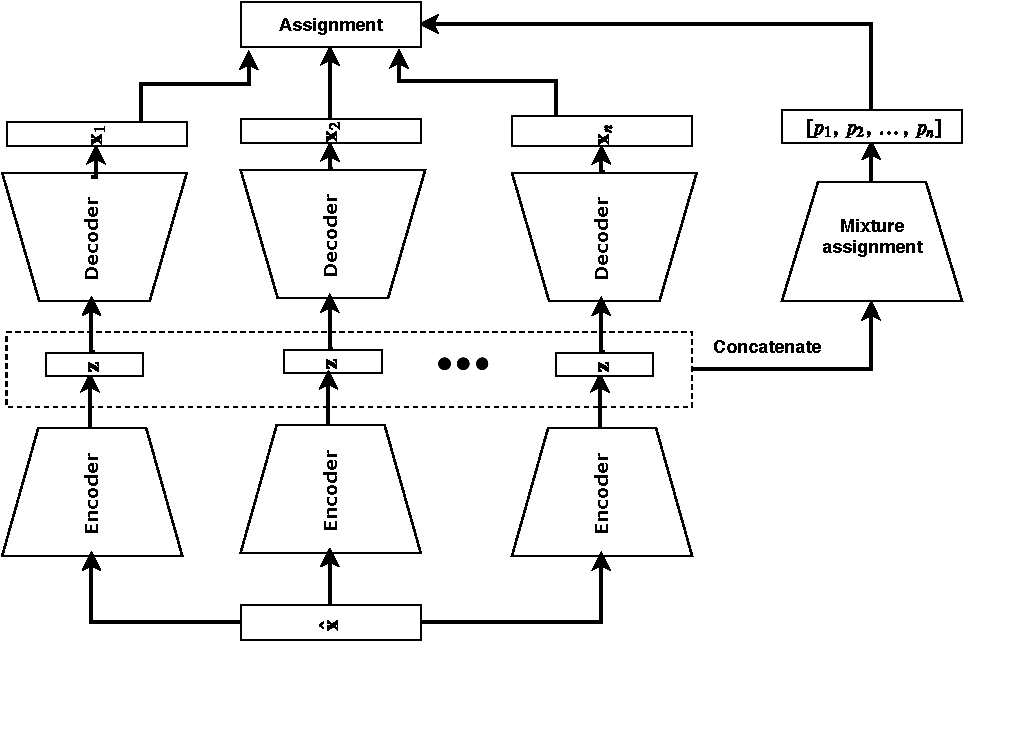
\includegraphics[width=.8\textwidth]{plots/mixae.pdf}
	\caption[Mixture of autoencoders schematic]{Schematic of a MIXAE model. A sample $\hat{\boldsymbol{x}}$ is compressed to set of lower-dimensional representations $\{\boldsymbol{z}^{(i)}\}$ by $N$ autoencoders. These samples are concatenated and passed through an auxiliary assignment network that predicts a confidence of cluster belonging for each autoencoder. For further details see the text. Figure adapted from \citet{Zhang}}
	\label{fig:mixae}
\end{figure}
{\color{blue} This section ends quite abruptly -MPK}


\subsection{Measuring performance}

We measure the performance of the clustering algorithms by two functions: clustering accuracy and the adjusted rand index (ARI). 
Ordinarily, we define accuracy as the agreement between a set of class predictions and their ground truth labels. 
However, with a clustering algorithm, there is no a priori knowledge of which cluster represents what ground-truth class. 
Since, in this example, we have access to ground-truth labels, we can define a clustering accuracy by calculating the maximum accuracy achieved by permuting which cluster should indicate a given class. 
A measure of clustering accuracy falls in the $[0, 1]$ range where $1$ denotes perfect agreement.  

Since we have access to ground truth labels, we can also calculate the ARI, which  measures the agreement between two sets of labels but {\color{blue}adjusts for chance assignments:: define this mathematically} \cite{Hubert1985}.
{\color{blue}  The effect is that a trivial clustering algorithm which predicts only one label will evaluate to ARI$=0$, but will have a nonzero accuracy:: need the math for this to be clear}.
As with the clustering accuracy, an ARI score is bounded in the range $[0, 1]$ where $1$ denotes perfect agreement.
%We refer to \citet{Hubert1985} for a detailed consideration of the ARI.

The performance is measured by comparing model predictions on the labelled subset of data (see table \ref{tab:datasets}) of the ARI.


\section{Results and Discussions}\label{sec:results}

The principal challenge in the AT-TPC experiments that we are trying to address is the reliance on labelled samples in the analysis, as future experiments may not have as visually dissimilar reaction products as we observe in the ${}^{46}$Ar experiment.  The ability to label data in the the ${}^{46}$Ar experiment does, however, provide a useful example where we can then explore unsupervised techniques. 

We first explore the results of applying a K-means approach on the latent space of a pre-trained network. Subsequently, we investigate the performance of the MIXAE algorithm as outlined in section \ref{sec:mixae}.

\subsection{K-means clustering on the VGG16 latent space}

The results of the clustering runs are included in table \ref{tab:clstr_vgg}. We observe that we are able to attain near-perfect clustering on simulated data and that there is a sharp decline in performance as we add noise by moving to the filtered and raw datasets. 


\begin{table}[H]
\centering 
\caption[K-means on pre-trained model]{K-means clustering results on AT-TPC event data. We observe that the performance predictably decreases with the amount of noise in the data.}\label{tab:clstr_vgg}
\begin{tabular}{lll}
\toprule
{} & Accuracy &   ARI \\
\midrule
Simulated &     0.97 &  0.89 \\
Filtered  &     0.74 &  0.39 \\
Raw       &     0.59 &  0.17 \\
\bottomrule
\end{tabular}

\end{table}

{\color{blue} This section may contain info that you can move to the metrics section??}
In addition to the performance measures reported in table \ref{tab:clstr_vgg}, it is interesting to observe which samples are wrongly assigned. To investigate this problem, we tabulate the assignments of samples relative to their ground truth labels. From these tables, we can infer which classes are more or less entangled with others. The results for each dataset is shown in figures \ref{fig:clster_confmat_sim} \ref{fig:clster_confmati_filt} and \ref{fig:clster_confmati_raw}. We observe that the proton class is consistently assigned in a pure cluster. Purity is inferred by how much spread there is in the column between the ground truth labels. A high-quality cluster will, in addition to being pure, also capture most entries the class represented by the cluster. For example, consider the row corresponding to the proton class in figure \ref{fig:clster_confmati_filt}. The column corresponding to the largest entry in the proton row has zero other predicted classes in it. From this, we conclude that the proton cluster is a high quality, high purity cluster. 

This high-quality cluster also appears in the clustering of raw data. From figure \ref{fig:clster_confmati_raw}, we observe that there is a high purity proton cluster. In contrast to the filtered data we observe that the deterioration in performance can largely be ascribed to the algorithm creating a proton + other cluster and a carbon + other cluster.

\begin{figure}
\centering
	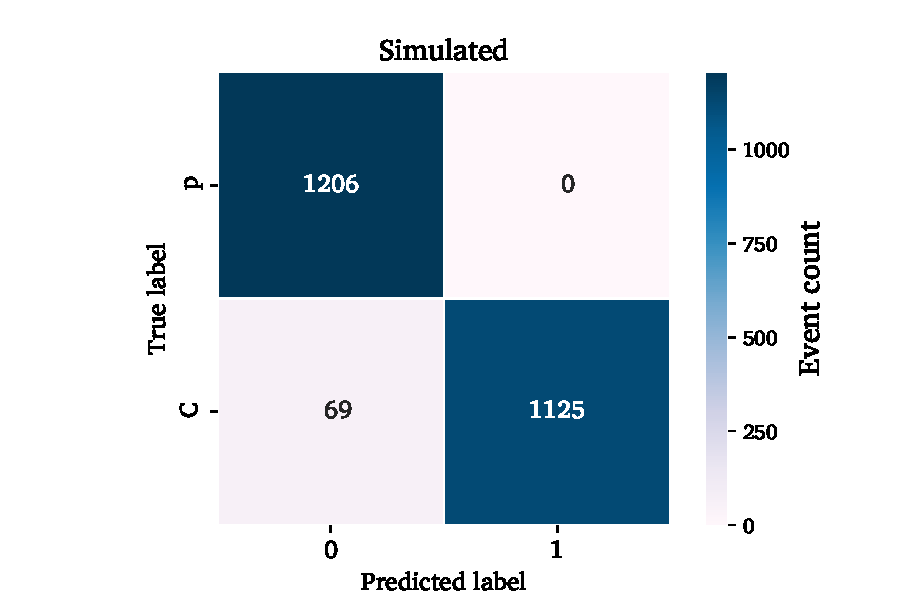
\includegraphics[width=\textwidth]{custom_work/Simulatedvgg_conf_mat.pdf} 
	\caption[Pre-trained network - confusion matrices]{Confusion matrix for the K-means clustering of simulated AT-TPC events. The true labels indicate samples belonging to the p (proton), or the carbon (C) class}\label{fig:clster_confmat_sim}
\end{figure}

\begin{figure}
\centering
	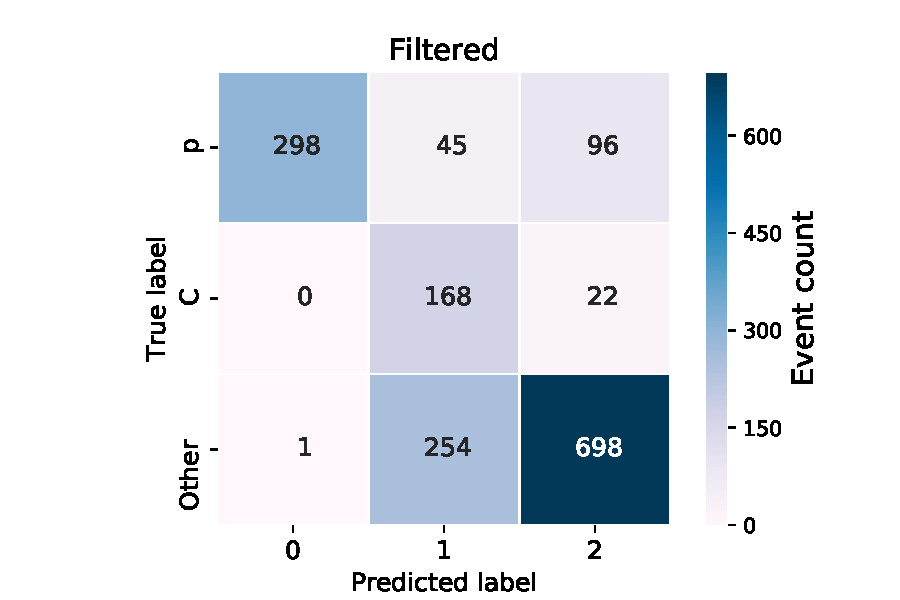
\includegraphics[width=\textwidth]{custom_work/Filteredvgg_conf_mat.pdf}
	\caption[Pre-trained network - confusion matrices]{Confusion matrix for the K-means clustering of filtered AT-TPC events. The true labels indicate samples belonging to the p (proton), carbon (C), or other classes. }\label{fig:clster_confmati_filt}
\end{figure}

\begin{figure}
	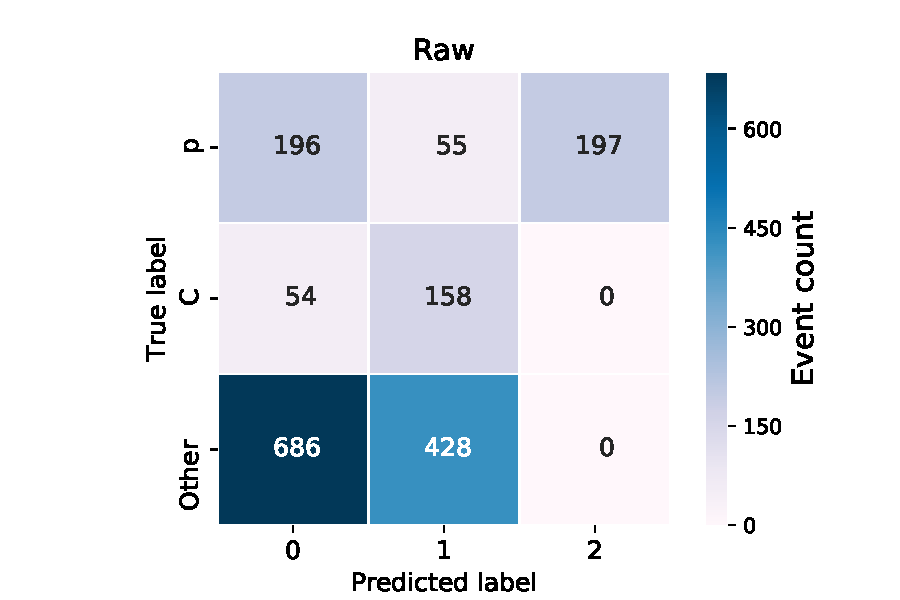
\includegraphics[width=\textwidth]{custom_work/Rawvgg_conf_mat.pdf}
\caption[Pre-trained network - confusion matrices]{Confusion matrix for the K-means clustering of raw AT-TPC events. The true labels indicate samples belonging to the p (proton), carbon (C), or other classes. }\label{fig:clster_confmati_raw}
\end{figure}


We repeat this analysis using a Principle Component Analysis (PCA) dimensionality reduction\footnote{
PCA is a common techinque to find the significant variations in data by projecting the data along a subset of its covariance matrix eigenvectors \cite{Marsland2009}
} on the latent space of the VGG16 model. This is done to estimate to what degree the class separating information is encoded in the entirety of the latent space, or in some select regions. The results from the PCA analysis {\color{blue} using the top XX principal components} were virtually identical to the results sans the PCA, indicating that a lower-dimensional encoding of the data is sufficient for data clustering for this experiment.
%and so we omit them for brevity. 

To further investigate the clusters presented in the matrix in figures \ref{fig:clster_confmati_filt} and \ref{fig:clster_confmati_raw}, we sample examples from the proton samples belonging to different clusters for the filtered and full data.
We display these examples in figures \ref{fig:filtered_vgg_clster_repr} and \ref{fig:full_vgg_clster_repr} respectively. Form these figures we gleam that the more noisy proton events are being clustered together with the amorphous other class. This is in line with the intuitive expectation from viewing the clustering tables in figures \ref{fig:clster_confmati_filt} and \ref{fig:clster_confmati_raw}.

\begin{figure}
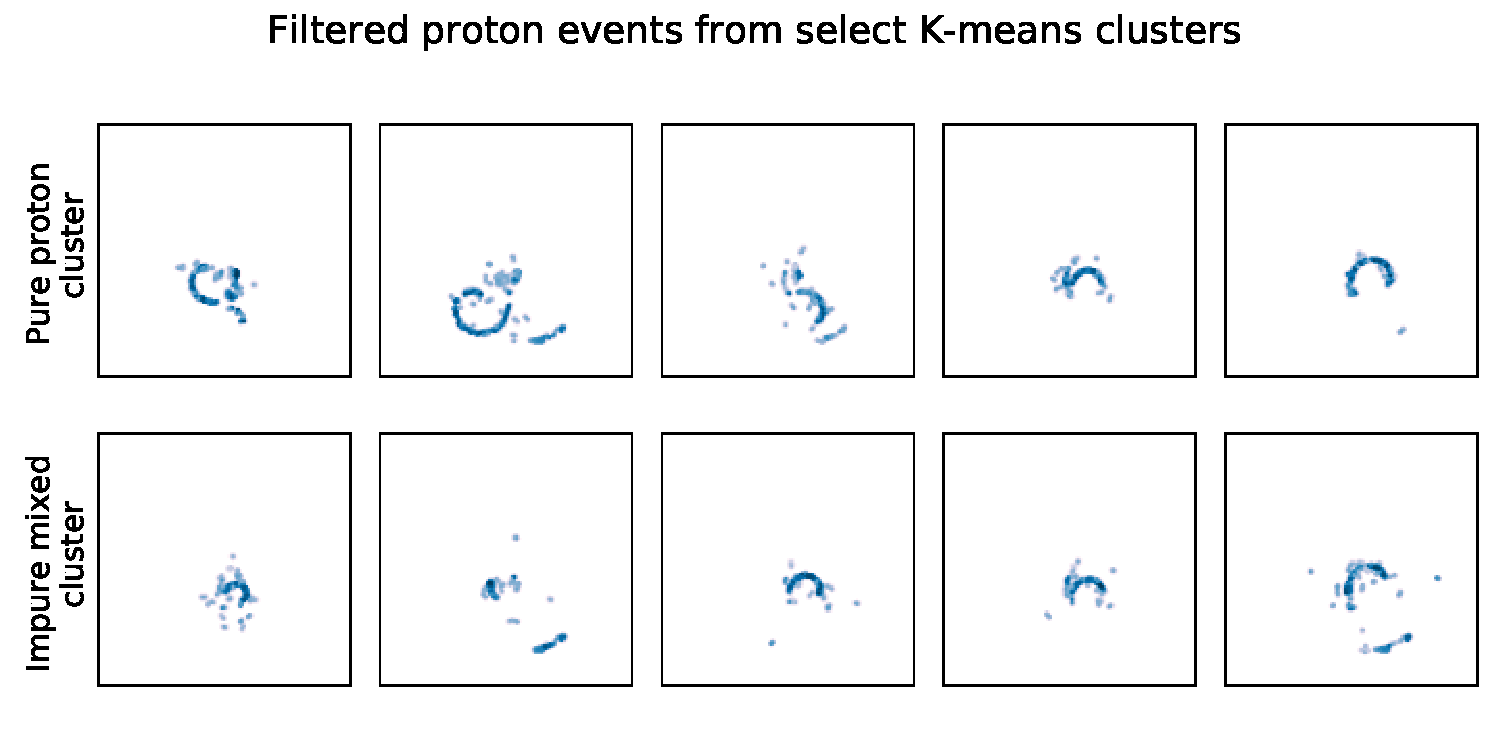
\includegraphics[width=\textwidth]{custom_work/Filteredexamples.pdf}
\caption[Filtered proton samples by cluster belonging]{Illustrating a sample of proton events from different K-means clusters from the filtered dataset. Each row belongs to a single cluster corresponding to the filtered confusion matrix in figure \ref{fig:clster_confmati_filt}}\label{fig:filtered_vgg_clster_repr}
\end{figure} 

\begin{figure}
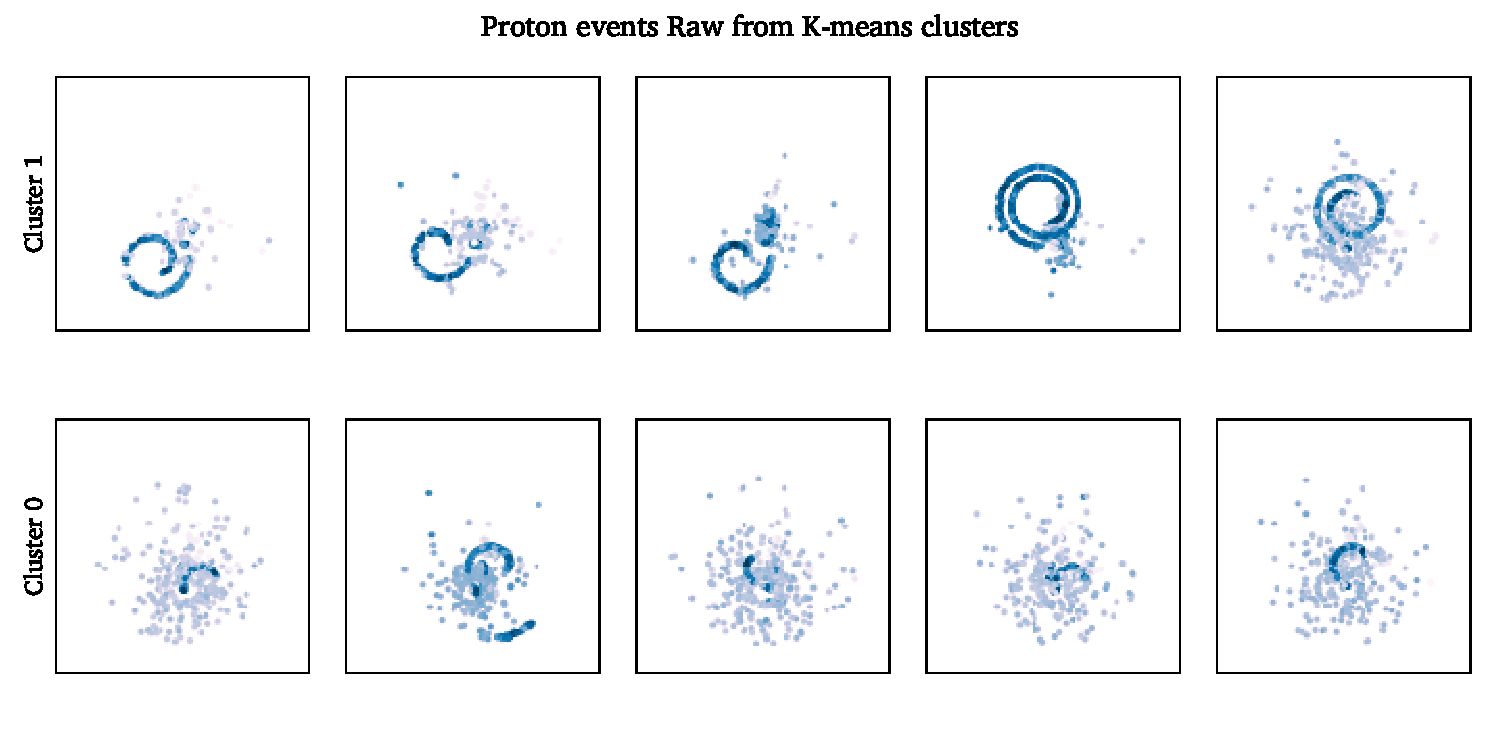
\includegraphics[width=\textwidth]{custom_work/Rawexamples.pdf}
\caption[Full proton samples by cluster belonging]{Illustrating a sample of proton events from different K-means clusters from the raw dataset. Each row belongs to a single cluster corresponding to the full confusion matrix in figure \ref{fig:clster_confmati_raw}}\label{fig:full_vgg_clster_repr}
\end{figure} 


\subsection{MIXAE clustering results}

In the previous section we demonstrated a powerful, but rather naive, clustering technique for AT-TPC track identification. To build on this result we will in this section explore the application of the mixture of autoencoders (MIXAE) algorithm introduced in section \ref{sec:mixae}.
For details on hyper-parameter tuning and the experimental procedure for training the MIXAE algorithm see appendix \ref{ax: mixae}

After hyperparameter tuning, each highest performing model is run $10$ times. The results are listed in table \ref{tab:clstr_mixae}.
We observe that, while the algorithm can achieve very strong performance, the performance varies. In some cases the MIXAE model converges to a seemingly good configuration, based on its unsupervised training goals. However, when inspecting its clustering performance against labelled data that seemingly good model does no better than random. 
This happens more frequently with raw data, indicating an interaction with the noise levels present in the events. 
 
\begin{table}[H]
\centering 
\caption[MIXAE clustering performance]{MIXAE clustering performance on the ${}^{46} Ar$ experimental data. In contrast with the VGG-16 + K-means approach we observe  significant variations in performance.}\label{tab:clstr_mixae}
\begin{tabular}{lllll}
\toprule
{} & \multicolumn{2}{c}{Accuracy} &   \multicolumn{2}{c}{ARI} \\
\midrule
{} & Top 1 &  $\mu \pm \sigma$ init $= 1$ & Top 1 & $\mu \pm \sigma$ \\
Simulated &  0.96 &  $0.74 \pm 0.16 $  & 0.84 &  $0.33 \pm 0.32 $\\
Filtered  & 0.75 &  $0.71 \pm 0.04 $ & 0.52 &  $0.38 \pm 0.14 $\\
Raw & 0.71 &  $0.61 \pm 0.07 $ &  0.32 &  $0.09 \pm 0.10 $   \\
\bottomrule
\end{tabular}
\end{table}

As with the VGG16 + KMeans approach we wish to further investigate the clustering results. Taking the best performing MIXAE model on filtered and raw data we tabulate the clusters against their labels. These tables are present in figures \ref{fig:mixae_confmat_filtered} and \ref{fig:mixae_confmat_raw} for filtered and raw data, respectively.

Applied to raw data the MIXAE captures a proton cluster in a similar vein to the K-means approach. The MIXAE forms a proton-majority cluster, but with a significant portion of the more noisy proton events being clustered with the other-class. Additionally, we do not observe the carbon events being separated from either the amorphous noise events or from the proton cluster. 

On filtered data the highest performing MiXAE model achieves strong separation of the other-class, but curiously creates two proton-majority clusters.
 
\begin{figure}
\centering
	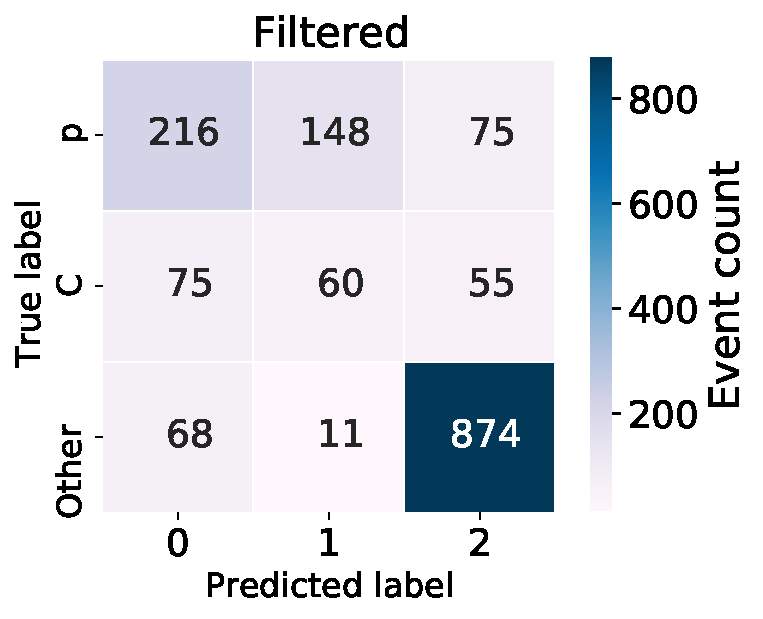
\includegraphics[width=\textwidth]{custom_work/Filtered_mixae_conf_mat.pdf}
\caption[MIXAE - confusion matrices]{Confusion matrix for the MIXAE clustering algorithm on filtered AT-TPC events. The true labels indicate samples belonging to the \texttt{p} (proton), \texttt{C} (Carbon), or \texttt{other} classes. We observe that the algorithm forms two proton-majority clusters, and one clearly defined cluster of the other events. }\label{fig:mixae_confmat_filtered}
\end{figure}

\begin{figure}
\centering
	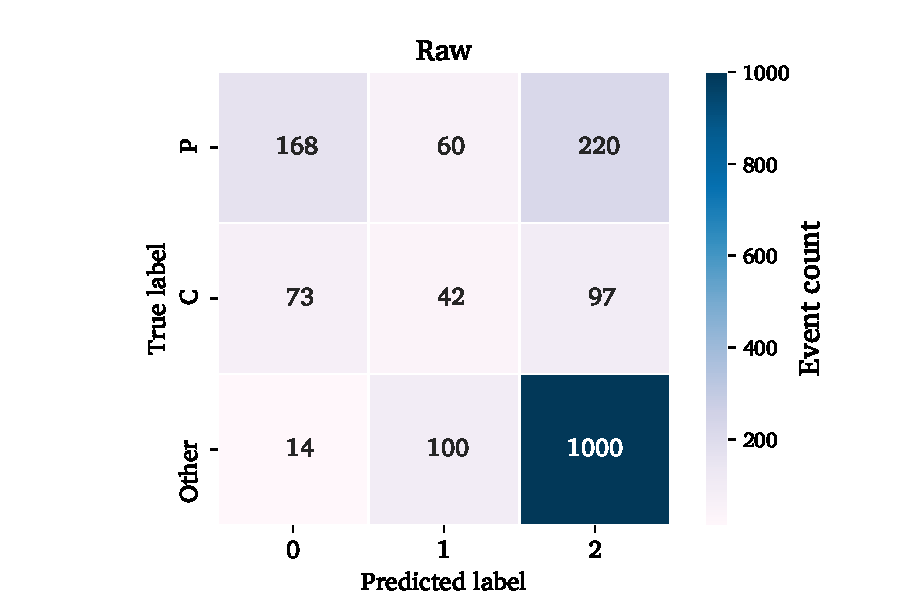
\includegraphics[width=\textwidth]{custom_work/Raw_mixae_conf_mat.pdf}
\caption[MIXAE - confusion matrices]{Confusion matrices for the MIXAE clustering algorithm on raw AT-TPC events. The true labels indicate samples belonging to the p (proton), carbon (C), or \texttt{other} classes. We observe that the algorithm correctly caputers a majority proton-event cluster in cluster 0. However, in contrast with the K-means approach this cluster is contaminated to some extend with both carbon and other events. }\label{fig:mixae_confmat_raw}
\end{figure}

\subsection{Performance comparison and ?????}

The most striking result we present in this work is the success of the K-means approach. As noted by \cite{Aggarwal} distance measures become less informative in higher dimensional spaces, but the K-means algorithm clusters events well in a very high-dimensional space.
Another surprise is the stability of the K-means algorithm. A stability we attribute to the quality of the VGG16 latent space in creating class-separating sub-spaces. While the separations are not perfect, the stability and quality of the proton track identification create solid empirical grounding for applying this approach to other active target experiments. 


It is also interesting to compare and contrast the clustering results from the MIXAE model with those of the VGG16$+$K-means. In particular, the discrepancy in stability is worth noting. While the top performing MIXAE runs outperform the K-means approach, its reliability suffers. However, the high performance achieved shines a light on valuable potential research into more bespoke models for unsupervised track identification.


\subsection{Alternative approaches}

In addition to the results presented in this section, we performed clustering with a number of different algorithms included in the \lstinline{scikit-learn} package. None of them provided any notable differences from the K-means results or were significantly worse. Notably, the DBSCAN algorithm \cite{Ester96adensity-based}\cite{Bergstra2012} failed to provide any useful clustering results. We find this important as one of the significant drawbacks of K-means, and the deep clustering algorithm presented in section \ref{sec:mixae}, is that they are all dependent on pre-determining the number of clusters. This is not the case for DBSCAN. 

Additionally, we considered the deep convolutional embedded clustering (DCEC) by \citet{Guo2017} as well as the MIXAE method introduced by \citet{Zhang}. While we were able to reproduce the authors' results on their data, the DCEC algorithm proved unable to cluster AT-TPC in our implementation. However, this provides valuable insight as the seeds of the clusters are constructed by a K-means algorithm. This insight contrasts with our positive results from applying a pre-trained model with k-means and highlights potentially significant differences in models trained on a supervised or unsupervised objective for clustering tasks in nuclear physics. 

\section{Conclusions and Perspectives}\label{sec{conclusion}}
% Begin edit by DB (6/17/2020)
The purpose of this study is to explore the application of unsupervised learning algorithms to event identification from an active target detector. The necessity to identify events from raw data prior to full processing is becoming a major issue in the data analysis of detectors with complex responses such as the AT-TPC.
As shown by both avenues explored in this work, it is clear that there is significant potential to eventually achieve event classification using fully automated unsupervised methods.

In particular, the ability of the K-means algorithm in picking out clear proton clusters from the VGG16 latent space lends itself well to an exploratory phase of analysis, where clusters of events corresponding to different reaction channels could be later identified by the experimenter.
Another interesting facet of the K-means clustering is its consistent performance. As shown in table \ref{tab:clstr_vgg}, the variance is zero for the performance metrics. This result indicates that the clusters are very clearly defined in the VGG16 latent space. However, as can be seen from the non-proton clusters in figures \ref{fig:clster_confmati_filt} and \ref{fig:clster_confmati_raw},  this does not necessarily imply that the physical signals are correspondingly clear. 
A caveat to the K-means method is that the number of clusters has to be specified in advance. Each experiment then has to be considered in light of possible reaction channels to determine a sensible number of clusters for this approach. 

The same caveat is present in the MIXAE implementation. While it shows better optimal performance than the K-means method, some inconsistencies were observed, that were notably not evident from the unsupervised training-objectives of the model. These two factors currently conspire to limit its immediate applicability, and more developments are needed for this approach. 

In summary, our study shows that unsupervised track classification with an implementation of the VGG16 + K-means approach is a viable solution. For future work, it is worth investigating whether the adaptation of bespoke models like the MIXAE algorithm will allow better performance at no significant cost to consistency.  
%Especially considering the flexibility to use 3D input representations or auxiliary physical goals in the optimization procedure. 
The two examples of unsupervised machine learning methods studied in this work are a first encouraging step towards automated classification of events that could not only greatly reduce the resource cost of analysis, but also eventually boost the efficiency of the experiment by allowing post-trigger decisions based on such algorithm implemented in hardware. Much progress remains to be done before achieving these goals.
% End edit by DB (6/17/2020)
%From our analysis it is clear that we are a ways off from a fully automated unsupervised method for track classification. {\color{orange}[flip this to positive ]} It is also clear that there is significant potential in both avenues explored in this work. 
%n particular, the surprising ability of the K-means algorithm in picking out clear proton clusters from the VGG16 latent space lends itself well to an exploratory phase of analysis.
%Another surprising facet of the K-means clustering is its consistent performance. As shown in table \ref{tab:clstr_vgg}, the variance is zero for the performance metrics. This result indicates that the clusters are very clearly defined in the VGG16 latent space. As we see from the non-proton clusters if figures \ref{fig:clster_confmati_filt} and \ref{fig:clster_confmati_raw}  that does not necessarily imply that the physical signals are correspondingly clear. 

%Additionally, a clear disadvantage to the K-means method is that the researcher has to specify the number of clusters in the data themselves. Each experiment then has to be considered in light of possible reaction channels to determine a sensible number of clusters for this approach. 

%The same weakness is present in the MIXAE implementation. Additionally, while it showed better optimal performance than the K-means method, it struggles with inconsistent results. This inconsistency was also notably not evident from the unsupervised training-objectives of the model. These two factors conspire to limit its immediate applicability. 

%In summary, we recommend that researchers performing unsupervised track classification begin with an implementation of the VGG16 + K-means approach. For future work, it is worth investigating whether the adaptations of bespoke models like the MIXAE algorithm will allow better performance at no significant cost to consistency.  Especially considering the flexibility to use 3D input representations or auxiliary physical goals in the optimization procedure. 


%{\color{orange}[RS Another abrupt end to a paragraph. Could probably use some rounding out.]} 

\appendix  
\section{VGG16}\label{app:vgg}
The choice of the kernel size is based on the fact that a stacked $3 \times 3$ kernel is equivalent to larger kernels in terms of the receptive field of the output. Three $3 \times 3$ kernels with stride $1$ have a $7 \times 7$ receptive field, but the larger kernel has $81\%$ more parameters and only one non-linearity \cite{Simonyan2014}. Stacking the smaller kernels then contributes to a lower computational cost. Additionally, there is a regularizing effect from the lowered number of parameters and increased explanatory power from the additional non-linearities.
\begin{table}
\caption[vgg architectures]{Showing the details of the VGG network architectures. Network D trained on the ImageNet \cite{Russakovsky2015} dataset the network known as  VGG16 and is what we use in this thesis.}\label{tab:vgg}
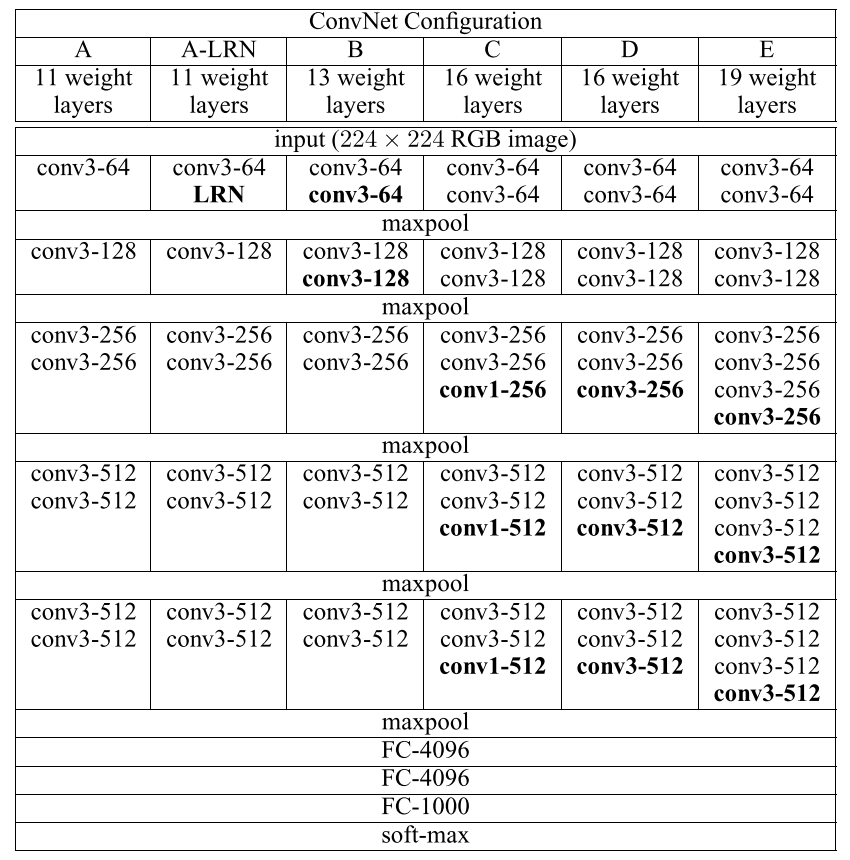
\includegraphics[width=\textwidth]{plots/vgg_architectures.png}
\end{table}

\section{MIXAE hyper-parameter tuning}\label{ax: mixae}

In the MIXAE algorithm the hyper-parameters to adjust are all the ordinary parameters that we introduced in table \ref{tab:convae_hyperparams}. In addition to those parameters we have the weighting of the loss terms: $\theta$, $\alpha$ and $\gamma$. These weighting parameters are attached to the reconstruction loss, sample entropy and batch-wise entropy respectively \cite{Zhang}. 
We focused on the tuning of the clustering hyper-parameters, and heuristically set the autoencoder hyper-parameters to a shallow $3\times3$ convolutional network.  

The parameters chosen for the autoencoders are listed in full in table \ref{tab:mixe_ae_hyperparams}.

To train the MIXAE clustering algorithm, we use the large simulated dataset with $M=80000$ points, evenly distributed between proton- and carbon-events. The algorithm is trained on a subset of $60000$ of these samples, and we track performance on the remaining $20000$ events. Since there are then only three remaining hyperparameters we choose to perform a coarse grid-search as described in section \ref{sec:hyperparam_search_arch}.Finally, for these parameters we re-ran the algorithm $N=10$ times to investigate the stability of the algorithm.

\begin{table}
\centering
\caption{Hyperparameter grid for the MIXAE loss weighting terms. The grid is given as exponents for logarithmic scales.}\label{tab:mixae_loss_weights}
\begin{tabular}{lll}
\toprule
Parameter & Grid & Scale \\
\midrule 
$\theta$ & $[-1,\, 5]$ & Logarithmic \\
$\alpha$ & $[-5,\, -1]$ & Logarithmic \\
$\gamma$ & $[3,\, 5]$ & Logarithmic
\end{tabular}
\end{table}

The grids selected for the search are listed in table \ref{tab:mixae_loss_weights}. The search yielded an optimal configuration with 

\begin{align}
\theta = 10^{-1}, \\
\alpha = 10^{-2}, \\
\gamma = 10^5.
\end{align}

For the full dataset the MIXAE hyperparameters converge to the same values as for the clean data:

\begin{align}
\theta &= 10^{1}, \\
\alpha &= 10^{-1}, \\
\gamma &= 3.162\times 10^3.
\end{align}

Lastly we supply the configuration used for the individual convolutional autoencoder networks in table \ref{tab:mixe_ae_hyperparams}

\begin{table}[H]
\renewcommand*{\arraystretch}{0.5}
\centering
\caption{Hyperparameters selected for the autoencoder components of the MIXAE algorithm, see table \ref{tab:convae_hyperparams} for a full description of the parameters.}\label{tab:mixe_ae_hyperparams}
\setlength{\extrarowheight}{15pt}
\hspace*{-0.5in}
\begin{tabular}{ll}
\toprule
Hyperparameter & Value \\
\midrule
\multicolumn{2}{l}{Convolutional parameters: } \\
\midrule
Number of layers & $4$ \\
Kernels & $[3,\,3,\,3,\,3]$\\
Strides & $[2,\,2,\,2,\,2]$ \\
Filters & $[64,\, 32, \,16, \,8,]$ \\ 
\midrule
\multicolumn{2}{l}{Network parameters: } \\
\midrule
Activation & LReLu \\
Latent dimension & 20  \\
Batchnorm & False \\
\midrule
\multicolumn{2}{l}{Optimizer parameters: } \\
\midrule
$\eta$ & $10^{-3}$ \\
$\beta_1$ & $0.9$ \\
$\beta_2$ & $0.99$ \\
\bottomrule
\end{tabular}
\end{table}


\bibliography{bibliography}
\end{document}
